\documentclass[12pt]{report}
\usepackage[utf8]{inputenc}
\usepackage[russian]{babel}
%\usepackage[14pt]{extsizes}
\usepackage{listings}
\usepackage{graphicx}
\usepackage{amsmath,amsfonts,amssymb,amsthm,mathtools} 
\usepackage{pgfplots}
\usepackage{filecontents}
\usepackage{indentfirst}
\usepackage{eucal}
\usepackage{enumitem}
\frenchspacing

\usepackage{indentfirst} % Красная строка


\usetikzlibrary{datavisualization}
\usetikzlibrary{datavisualization.formats.functions}

\usepackage{amsmath}




% Для листинга кода:
\lstset{ %
language=C++,                 % выбор языка для подсветки (здесь это С++)
basicstyle=\small\sffamily, % размер и начертание шрифта для подсветки кода
numbers=left,               % где поставить нумерацию строк (слева\справа)
numberstyle=\tiny,           % размер шрифта для номеров строк
stepnumber=1,                   % размер шага между двумя номерами строк
numbersep=5pt,                % как далеко отстоят номера строк от подсвечиваемого кода
showspaces=false,            % показывать или нет пробелы специальными отступами
showstringspaces=false,      % показывать или нет пробелы в строках
showtabs=false,             % показывать или нет табуляцию в строках
frame=single,              % рисовать рамку вокруг кода
tabsize=2,                 % размер табуляции по умолчанию равен 2 пробелам
captionpos=t,              % позиция заголовка вверху [t] или внизу [b] 
breaklines=true,           % автоматически переносить строки (да\нет)
breakatwhitespace=false, % переносить строки только если есть пробел
escapeinside={\#*}{*)}   % если нужно добавить комментарии в коде
}

\usepackage[left=2cm,right=2cm, top=2cm,bottom=2cm,bindingoffset=0cm]{geometry}
% Для измененных титулов глав:
\usepackage{titlesec, blindtext, color} % подключаем нужные пакеты
\definecolor{gray75}{gray}{0.75} % определяем цвет
\newcommand{\hsp}{\hspace{20pt}} % длина линии в 20pt
% titleformat определяет стиль
\titleformat{\chapter}[hang]{\Huge\bfseries}{\thechapter\hsp\textcolor{gray75}{|}\hsp}{0pt}{\Huge\bfseries}


% plot
\usepackage{pgfplots}
\usepackage{filecontents}
\usetikzlibrary{datavisualization}
\usetikzlibrary{datavisualization.formats.functions}

\begin{document}
%\def\chaptername{} % убирает "Глава"
\thispagestyle{empty}
\begin{titlepage}
	\noindent \begin{minipage}{0.15\textwidth}
	
\includegraphics[width=\linewidth]{report_files/bmstu_logo.jpg}
	\end{minipage}
	\noindent\begin{minipage}{0.9\textwidth}\centering
		\textbf{Министерство науки и высшего образования Российской Федерации}\\
		\textbf{Федеральное государственное бюджетное образовательное учреждение высшего образования}\\
		\textbf{~~~«Московский государственный технический университет имени Н.Э.~Баумана}\\
		\textbf{(национальный исследовательский университет)»}\\
		\textbf{(МГТУ им. Н.Э.~Баумана)}
	\end{minipage}
	
	\noindent\rule{18cm}{3pt}
	\newline\newline
	\noindent ФАКУЛЬТЕТ $\underline{\text{«Информатика и системы управления»}}$ \newline\newline
	\noindent КАФЕДРА $\underline{\text{«Программное обеспечение ЭВМ и информационные технологии»}}$\newline\newline\newline\newline\newline
	
	
	\begin{center}
		\noindent\begin{minipage}{1.3\textwidth}\centering
			\Large\textbf{  Отчет по лабораторной работе №1}\newline
			\textbf{по дисциплине "Анализ алгоритмов"}\newline\newline
		\end{minipage}
	\end{center}
	
	\noindent\textbf{Тема} $\underline{\text{Редакционные расстояния}}$\newline\newline
	\noindent\textbf{Студент} $\underline{\text{Костев Д.И.}}$\newline\newline
	\noindent\textbf{Группа} $\underline{\text{ИУ7-51Б}}$\newline\newline
	\noindent\textbf{Оценка (баллы)} $\underline{\text{~~~~~~~~~~~~~~~~~~~~~~~~~~~}}$\newline\newline
	\noindent\textbf{Преподаватели} $\underline{\text{Волкова Л.Л. }}$\newline\newline\newline
	
	\begin{center}
		\vfill
		Москва~---~\the\year
		~г.
	\end{center}
\end{titlepage}

\setcounter{page}{2}
\tableofcontents

\newpage
\chapter*{Введение}
\addcontentsline{toc}{chapter}{Введение}
\textbf{Расстояние Левенштейна} - минимальное количество операций вставки одного символа, удаления одного символа и замены одного символа на другой, необходимых для превращения одной строки в другую.
\newline

Расстояние Левенштейна применяется в теории информации и компьютерной лингвистике для следующих задач:
\begin{itemize}
	\item исправления ошибок в слове;
	\item сравнения текстовых файлов утилитой diff;
	\item в биоинформатике для сравнения генов, хромосом и белков.
\end{itemize}

\textbf{Цель лабораторной работы: } изучение метода динамического программирования на материале алгоритмов нахождения расстояния Левенштейна и Дамерау-Левенштейна.

\textbf{Для достижения поставленной цели требуется решить поставленные задачи.}
\begin{enumerate}
  	\item Изучение алгоритмов Левенштейна и Дамерау-Левенштейна.
	\item Применение метода динамического программирования для матричной реализации указанных алгоритмов.
	\item Получение практических навыков реализации указанных алгоритмов: матричные и рекурсивные версии.
	\item Сравнительный анализ линейной и рекурсивной реализаций выбранного алгоритма определения расстояния между строками по затрачиваемым ресурсам (времени и памяти).
	\item Экспериментальное определение различий во временнóй и емкостной эффективности реализаций алгоритмов.
\end{enumerate}

\chapter{Аналитическая часть}
\section{Расстояние Левенштейна}
Расстояние Левенштейна между двумя строками — это минимальное количество операций вставки, удаления и замены, необходимых для превращения одной строки в другую.


Цены операций могут зависеть от вида операции (вставка (insert), удаление (delete), замена (replace)) и/или от участвующих в ней символов, отражая разную вероятность разных ошибок при вводе текста, и т. п. В общем случае:

\begin{itemize}
	\item $w(a,b)$ — цена замены символа $a$ на символ $b$;
	\item $w(\lambda,b)$ — цена вставки символа $b$;
	\item $w(a,\lambda)$ — цена удаления символа $a$.
\end{itemize}

Для решения задачи о редакционном расстоянии необходимо найти последовательность замен, минимизирующую суммарную цену. Расстояние Левенштейна является частным случаем этой задачи при

\begin{itemize}
	\item $w(a,a)=0$,
	\item $w(a,b)=1, \medspace a \neq b$,
	\item $w(\lambda,b)=1$,
	\item $w(a,\lambda)=1$.
\end{itemize}

Расстояние Левенштейна между двумя строками a и b может быть вычислено по формуле \ref{eq:D}, где $|a|$ означает длину строки $a$; $a[i]$ — i-ый символ строки $a$ , функция $D(i, j)$ определена как:
\begin{equation}
\label{eq:D}
D(i, j) = \begin{cases}
0 &\text{i = 0, j = 0}\\
i &\text{j = 0, i > 0}\\
j &\text{i = 0, j > 0}\\
\min \lbrace \\
\qquad D(i, j-1) + 1\\
\qquad D(i-1, j) + 1 &\text{i > 0, j > 0}\\
\qquad D(i-1, j-1) + m(a[i], b[j]) &\text(\ref{eq:m})\\
\rbrace
\end{cases},
\end{equation}

а функция \ref{eq:m} определена как:
\begin{equation}
\label{eq:m}
m(a, b) = \begin{cases}
0 &\text{если a = b,}\\
1 &\text{иначе}
\end{cases}.
\end{equation}

Рекурсивный алгоритм реализует формулу \ref{eq:D}.
Функция $D$ составлена для решения следующих задач.
\begin{enumerate}
	\item Для перевода из пустой строки в пустую требуется ноль операций.
	\item Для перевода из пустой строки в строку $a$ требуется $|a|$ операций.
	\item Для перевода из строки $a$ в пустую требуется $|a|$ операций.
	\item Для перевода из строки $a$ в строку $b$ требуется выполнить последовательно некоторое количество операций (удаление, вставка, замена) в некоторой последовательности. Последовательность проведения любых двух операций можно поменять, порядок проведения операций не имеет никакого значения. Полагая, что $a', b'$  — строки $a$ и $b$ без последнего символа соответственно, цена преобразования из строки $a$ в строку $b$ может быть выражена как:
	\begin{itemize}
		\item сумма цены преобразования строки $a$ в $b$ и цены проведения операции удаления, которая необходима для преобразования $a'$ в $a$;
		\item сумма цены преобразования строки $a$ в $b$  и цены проведения операции вставки, которая необходима для преобразования $b'$ в $b$;
		\item сумма цены преобразования из $a'$ в $b'$ и операции замены, предполагая, что $a$ и $b$ оканчиваются разные символы;
		\item цена преобразования из $a'$ в $b'$, предполагая, что $a$ и $b$ оканчиваются на один и тот же символ.
	\end{itemize}
\end{enumerate}

	Минимальной ценой преобразования будет минимальное	значение приведенных вариантов.

\section{Расстояния Дамерау — Левенштейна}

Расстояние Дамерау — Левенштейна может быть найдено по формуле (\ref{eq:d}):

\begin{equation}
\label{eq:d}
d_{a,b}(i, j) = \begin{cases}
\max(i, j), &\text{если }\min(i, j) = 0,\\
\min \lbrace \\
\qquad d_{a,b}(i, j-1) + 1,\\
\qquad d_{a,b}(i-1, j) + 1,\\
\qquad d_{a,b}(i-1, j-1) + m(a[i], b[j]), &\text{иначе}\\
\qquad \left[ \begin{array}{cc}d_{a,b}(i-2, j-2) + 1, &\text{если }i,j > 1;\\
\qquad &\text{}a[i] = b[j-1]; \\
\qquad &\text{}b[j] = a[i-1]\\
\qquad \infty, & \text{иначе}\end{array}\right.\\
\rbrace
\end{cases}.
\end{equation}

Формула выводится по тем же соображениям, что и формула (\ref{eq:D}).
Как и в случае с рекурсивным методом, прямое применение этой формулы неэффективно по времени исполнения, то аналогично методу из \ref{sec:recmat} производится добавление матрицы для хранения промежуточных значений рекурсивной формулы.



\section{Матричный алгоритм нахождения расстояния Левенштейна}

Прямая реализация формулы \ref{eq:D} может быть малоэффективна по времени исполнения при больших $i, j$, т. к. множество промежуточных значений $D(i, j)$ вычисляются заново множество раз подряд. Для оптимизации нахождения расстояния Левенштейна можно использовать матрицу в целях хранения соответствующих промежуточных значений (выполнять меморизацию промежуточных значений). В таком случае алгоритм представляет собой построчное заполнение матрицы $A_{|a|,|b|}$ значениями $D(i, j)$.


\section{Рекурсивный алгоритм нахождения расстояния Левенштейна с заполнением матрицы}

\label{sec:recmat}


Рекурсивный алгоритм заполнения можно оптимизировать по времени выполнения с использованием матричного алгоритма. Суть данного метода заключается в параллельном заполнении матрицы при выполнении рекурсии. В случае, если рекурсивный алгоритм выполняет расчёт для данных, которые еще не были обработаны (в ячейке матрицы записана машиная бесконечность), результат нахождения расстояния заносится в матрицу. В случае, если обработанные ранее данные встречаются снова (в ячейке матрицы находится значение, отличное от машинной бесконечности), для них расстояние не находится и алгоритм переходит к следующему шагу.

\section{Вывод из аналитической части}
	В данном разделе были рассмотрены алгоритмы нахождения расстояния Левенштейна и Дамерау-Левенштейна, который является модификацией первого, учитывающего возможность перестановки соседних символов. Формулы Левенштейна и Дамерау — Левенштейна для рассчета расстояния между строками задаются рекурсивно, а следовательно, алгоритмы могут быть реализованы рекурсивно или итерационно.
	
\clearpage

\chapter{Конструкторская часть}

\section{Схемы алгоритмов}
В данной части будут рассмотрены схемы алгоритмов нахождения расстояние Левештейна и Дамерау - Левенштейна. На рисунках 2.1 - 2.4 представлены рассматриваемые алгоритмы.\newline

\begin{figure}[hp!]
	\centering
	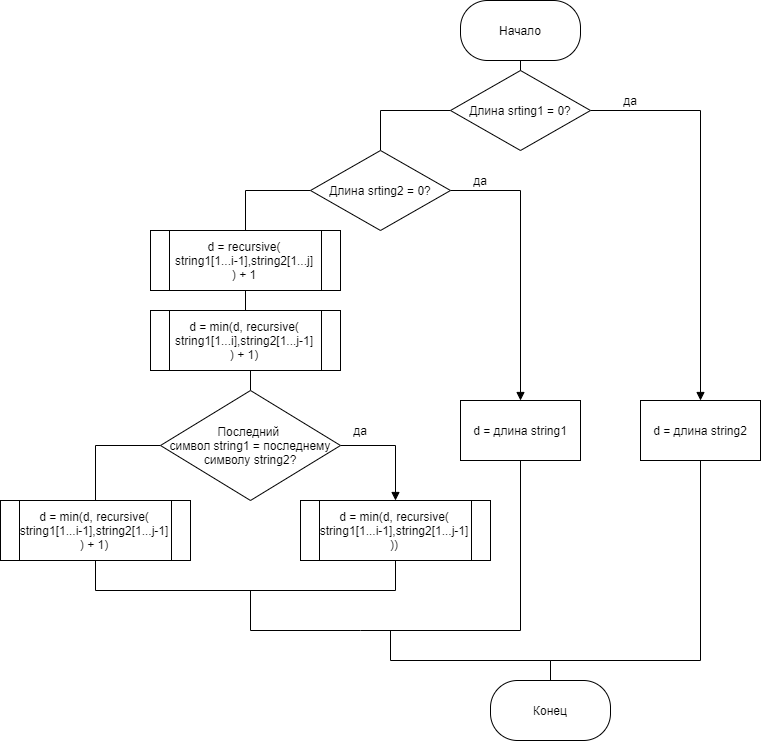
\includegraphics[width=0.85\linewidth]{report_files/recursive_levenshtein.png}
	\caption{Схема рекурсивного алгоритма нахождения расстояния Левенштейна}
	\label{fig:mpr}
\end{figure}

\begin{figure}[hp!]
	\centering
	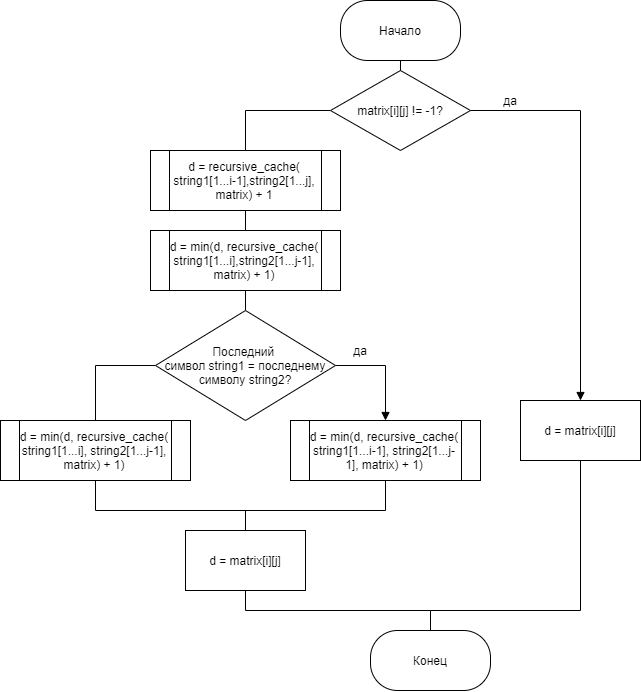
\includegraphics[scale=0.8]{report_files/memorize_recursive_levenshtein.png}
	\caption{Схема рекурсивного алгоритма с меморизацией значений расстояния Левенштейна}
	\label{fig:mpr}
\end{figure}

\begin{figure}[hp!]
	\centering
	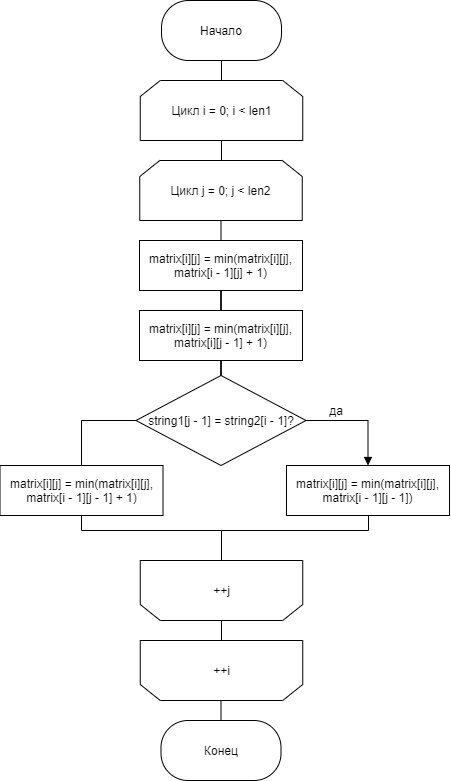
\includegraphics[scale=0.75]{report_files/iteration_levenshtein.png}
	\caption{Схема итеративного алгоритма нахождения расстояния Левенштейна}
	\label{fig:mpr}
\end{figure}

\begin{figure}[hp!]
	\centering
	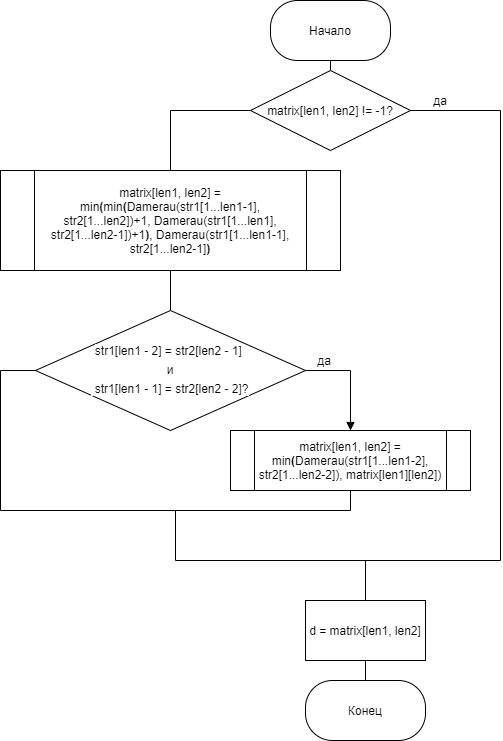
\includegraphics[scale=0.75]{report_files/recursive_damerau_levenshtein.png}
	\caption{Схема итеративного алгоритма нахождения расстояния Дамерау-Левенштейна}
	\label{fig:mpr}
\end{figure}

\newpage
\section{Вывод из конструкторской части}
	На основе теоретических данных, полученные в аналитическом разделе, были построены схемы рассматриваемых алгоритмов.

\chapter{Технологическая часть}

\section{Требование к ПО}
Ко вводу предъявляются следующие требования.
\begin{enumerate}
	\item На вход подаются две строки в любой раскладке (в том числе и пустые).
	\item ПО должно выводить полученное расстояние и вспомогательны матрицы.
	\item ПО должно выводить потраченную память и время.
\end{enumerate}

\section{Средства реализации}
Для реализации программы нахождения расстояние Левенштейна был выбран язык программирования c++. Для анализа времени использовалась функция getProcessTimes \cite{bibGetProcessTimes}.

\section{Реализация алгоритмов}

В листингах 3.1 - 3.4 приведена реализация алгоритмов нахождения расстояния Левенштейна и Дамерау-Левенштейна.

\begin{lstlisting}[label=some-code,caption=Функция нахождения расстояния Левенштейна рекурсивно,language=C++]
size_t recur(const string &str1, const size_t len1, const string &str2, const size_t len2)
{
    if (len1 == len2 && len1 == 0)
        return 0;
    else if (len1 == 0)
        return len2;
    else if (len2 == 0)
        return len1;
    else
    {
        bool flag = str1[len1 - 1] != str2[len2 - 1];
        return min(min(recur(str1, len1 - 1, str2, len2) + 1,
                       recur(str1, len1, str2, len2 - 1) + 1),
                   recur(str1, len1 - 1, str2, len2 - 1) + flag);
    }
}
\end{lstlisting}

\begin{lstlisting}[label=some-code,caption=Функция нахождения расстояние Левенштейна рекурсивно с меморизацией,language=C++]
size_t rec_cache(const string &str1, const size_t len1, const string &str2, const size_t len2, size_t **matr)
{
    if (matr[len1][len2] != 0)
        return matr[len1][len2];
    else if (len1 == len2 && len1 == 0)
        matr[len1][len2] = 0;
    else if (len1 == 0)
        matr[len1][len2] = len2;
    else if (len2 == 0)
        matr[len1][len2] = len1;
    else
    {
        bool flag = str1[len1 - 1] != str2[len2 - 1];
        matr[len1][len2] = min(min(rec_cache(str1, len1 - 1, str2, len2, matr) + 1,
                                   rec_cache(str1, len1, str2, len2 - 1, matr) + 1),
                               rec_cache(str1, len1 - 1, str2, len2 - 1, matr) + flag);
    }
    return matr[len1][len2];
}

size_t rec_cache_method(const string &str1, const string &str2)
{
    size_t len1 = str1.length(), len2 = str2.length();
    auto matr = new size_t *[len1 + 1];
    for (size_t i = 0; i < len1 + 1; i++)
        matr[i] = new size_t[len2 + 1];
    for (size_t i = 0; i < len1 + 1; i++)
        for (size_t j = 0; j < len2 + 1; j++)
            matr[i][j] = 0;

    rec_cache(str1, len1, str2, len2, matr);
    size_t result = matr[len1][len2];
    for (size_t i = 0; i < len1 + 1; i++)
        delete matr[i];
    delete matr;
    return result;
}
\end{lstlisting}

\begin{lstlisting}[label=some-code,caption=Функция нахождения расстояния Левенштейна итеративно,language=C++]
size_t matr_method(const string &str1, const string &str2)
{
    size_t n = str1.length() + 1, m = str2.length() + 1;
    auto matr = new size_t *[n];
    for (size_t i = 0; i < n; i++) 
    {
        matr[i] = new size_t[m];
        matr[i][0] = i;
    }
    for (size_t i = 0; i < m; i++)
        matr[0][i] = i;

    for (size_t i = 1; i < n; i++)
        for (size_t j = 1; j < m; j++)
            matr[i][j] = min(min(matr[i - 1][j] + 1, matr[i][j - 1] + 1), matr[i - 1][j - 1] + (str1[i - 1] == str2[j - 1] ? 0 : 1));

    size_t result = matr[n - 1][m - 1];
    for (size_t i = 0; i < n; i++)
        delete matr[i];
    delete matr;
    return result;
}
\end{lstlisting}


\begin{lstlisting}[label=some-code,caption=Функция нахождения расстояния Дамерау-Левенштейна матрично,language=C++]
size_t Damerau(const string &str1, const size_t len1, const string &str2, const size_t len2, size_t **matr)
{
    if (matr[len1][len2] != 0)
        return matr[len1][len2];
    else if (len1 == len2 && len1 == 0)
        matr[len1][len2] = 0;
    else if (len1 == 0)
        matr[len1][len2] = len2;
    else if (len2 == 0)
        matr[len1][len2] = len1;
    else 
    {
        bool flag = str1[len1 - 1] != str2[len2 - 1];
        matr[len1][len2] = min(min(Damerau(str1, len1 - 1, str2, len2, matr) + 1,
                                   Damerau(str1, len1, str2, len2 - 1, matr) + 1),
                               Damerau(str1, len1 - 1, str2, len2 - 1, matr) + flag);

        if (len1 > 1 && len2 > 1 && str1[len1 - 2] == str2[len2 - 1] && str1[len1 - 1] == str2[len2 - 2])
            matr[len1][len2] = min(Damerau(str1, len1 - 2, str2, len2 - 2, matr) + 1, matr[len1][len2]);
    }
    return matr[len1][len2];
}

size_t Damerau_method(const string &str1, const string &str2)
{
    size_t len1 = str1.length(), len2 = str2.length();
    auto matr = new size_t *[len1 + 1];
    for (size_t i = 0; i < len1 + 1; i++)
        matr[i] = new size_t[len2 + 1];
    for (size_t i = 0; i < len1 + 1; i++)
        for (size_t j = 0; j < len2 + 1; j++)
            matr[i][j] = 0;

    Damerau(str1, len1, str2, len2, matr);

    size_t result = matr[len1][len2];
    for (size_t i = 0; i < len1 + 1; i++)
        delete matr[i];
    delete matr;
    return result;
}

\end{lstlisting}

\section{Тестовые данные}

В таблице 3.1 приведены тестовые данные, на которых было протестированно разработанное ПО. Тестирование проводилось по методу черного ящика. Все тесты пройдены успешно.
\begin{table}[hp!]
	\begin{center}
		\caption{Тестовые данные}
		\newline
		\begin{tabular}{|c c c c c|} 
			\hline
			№ & Первое слово & Второе слово & Ожидаемый результат & Полученный результат \\ [0.8ex] 
			\hline
			1 &  &  & 0 0 0 0 & 0 0 0 0\\
			\hline
			2 & kot & skat & 2 2 2 2 & 2 2 2 2\\
			\hline
			3 & kate & ktae & 2 2 1 1 & 2 2 1 1\\
			\hline
			4 & abacaba & aabcaab & 4 4 2 2 & 4 4 2 2\\
			\hline
			5 & sobaka & sboku & 3 3 3 3 & 3 3 3 3\\
			\hline
			6 & qwerty & queue & 4 4 4 4 & 4 4 4 4\\
			\hline
			7 & aaaa & bbbbb & 5 5 5 5  & 5 5 5 5\\
			\hline
			8 &  & abc & 3 3 3 3 & 3 3 3 3\\
			\hline
			9 & parallels &  & 9 9 9 9 & 9 9 9 9\\
			\hline
			10 & буквы & букыв & 2 2 2 1 & 2 2 2 1\\
			\hline
		\end{tabular}
	\end{center}
\end{table}
\newline

\section{Вывод из технологической части}
В данном разделе были разработаны исходные коды четырех алгоритмов: вычисления расстояния Левенштейна рекурсивно, с заполнением матрицы и рекурсивно с заполнением матрицы, а также вычисления расстояния Дамерау — Левенштейна с заполнением матрицы.

\chapter{Исследовательская часть}

\section{Технические характеристики}

Ниже приведеные технические характеристики устройства, на котором было проведенно тестирование ПО.

\begin{itemize}

	\item Операционная система: Windows 10 64-bit.

	\item Оперативная память: 8 ГБ.

	\item Процессор: Intel(R) Core(TM) i5-8250 CPU @ 1.60GHz.

\end{itemize}

\section{Время выполнения алгоритмов}
Время выполнения алгоритм замерялось с помощью применения технологии профайлинга. Данный инстрмуент даёт детальное описание количества вызовов и количества времени CPU, занятого каждой функцией. \newline

В таблице 4.1. представленны замеры времени работы для каждого из алгоритмов. Рекурсивный алгоритм проводился на строках размером до 10 символов, из-за слишком быстрого увеличения времени работы программы с увеличением длины строки.

\begin{table} [h!]
	\caption{Таблица времени выполнения алгоритмов (в милисекундах)}
	\begin{center}
		\begin{tabular}{|c c c c c|} 
		 	\hline
			Длина строки & Итеративный & Рекурсивный & Рек. с меморизацией & Дамерау-Левенштейн \\
		 	\hline
		 	5 & 0.00078125 & 0.03125 & 0.00109375 & 0.00125\\
		 	6 & 0.0009375 & 0.078125 & 0.0015625 & 0.00171875\\
		 	7 & 0.00125 & 0.4375 & 0.00203125 & 0.00203125\\
		 	8 & 0.0015625 & 2.3125 & 0.0028125 & 0.0028125\\
		 	9 & 0.0021875 & 13.625 & 0.00328125 & 0.0034375\\
		 	10 & 0.003125 & -- & 0.0046875 & 0.0046875\\
		 	20 & 0.0078125 & -- & 0.0171875 & 0.015625 \\
			30 & 0.0171875 & -- & 0.028125 & 0.0328125 \\
			40 & 0.0234375 & -- & 0.046875 & 0.05625 \\
			50 & 0.0421875 & -- & 0.078125 & 0.084375 \\
			\hline
		\end{tabular}
	\end{center}
\end{table}

\section{Использование памяти}

Алгоритмы нахождения расстояния Левенштейна и Дамерау — Левенштейна не отличаются друг от друга с точки зрения использования памяти.

Максимальная глубина стека вызовов при рекурсивной реализации равна сумме длин входящих строк. Поэтому, максимальный расход памяти равен: 

\begin{equation}
(\mathcal{S}(STR_1) + \mathcal{S}(STR_2)) \cdot (2 \cdot \mathcal{S}\mathrm{(string)} + 3 \cdot \mathcal{S}\mathrm{(integer)}),
\end{equation}

\noindent где $\mathcal{S}$ — оператор вычисления размера, $STR_1$, $STR_2$ — строки, $\mathrm{string}$ — строковый тип, 

\noindent $\mathrm{integer}$ — целочисленный тип.

Использование памяти при итеративной реализации теоретически равно:
\begin{equation}
(\mathcal{S}(STR_1) + 1) \cdot (\mathcal{S}(STR_2) + 1) \cdot \mathcal{S}\mathrm{(integer)} + 5\cdot \mathcal{S}\mathrm{(integer)} + 2 \cdot \mathcal{S}\mathrm{(string)}.
\end{equation}


\section{Вывод из исследовательской части}

Рекурсивная реализация алгоритма нахождения расстояния Левенштейна работает дольше итеративной реализации, время работы этой реализации увеличивается в геометрической прогрессии. Рекурсивный с матрицей и Дамерау-Левенштейна работают примерно за одно время и лишь немного уступают итеративному алгоритму.


\chapter*{Заключение}
\addcontentsline{toc}{chapter}{Заключение}

В ходе проделанной работы были выполнены следующие задачи.
\begin{enumerate}
    \item Был изучен метод динамического программирования на материале реализации алгоритмов нахождения расстояния Левенштейна и Дамерау-Левенштейна.
    \item Были изучены алгоритмы поиска расстояния Левенштейна и Дамерау-Левенштейна нахождения расстояния между строками.
    \item Получены практические навыки раелизации указанных алгоритмов в матричной и рекурсивных версиях, а так же в версиях с мемоизацией.
    \item Был произведен сравнительный анализ линейной и рекурсивной реализаций выбранного алгоритма определения расстояния между строками по затрачиваемым ресурсам (времени и памяти).
    \item Экспериментально было подтверждено различие во временной эффективности рекурсивной и нерекурсивной реализаций выбранного алгоритма определения расстояния между строками при помощи разработаного программного обеспечения на материале замеров процессорного времени выполнения реализации на варьирующихся длинах строк. 
\end{enumerate}

Рекурсивная реализация алгоритма Левенштейна проигрывает нерекурсивной по времени исполнения в несколько десятков раз. Так же стоит отметить, что итеративный алгоритм Левештейна выполняется немного быстрее, чем итеративный алгоритм Дамерау - Левенштейна, но в целом алгоритмы выполняются за примерно одинаковое время.

Теоретически было рассчитано использования памяти в каждой из реализаций алгоритмов нахождения расстояния Левенштейна и Дамерау - Левенштейна. Алгоритм итеративный использует несколько большее количество памяти.

Из этого можно сделать вывод: если требуется самый быстрое решение задачи, то нужно использовать итеративный алгоритм, если же нужно сберечь память - Дамерау-Левенштейна.
\newpage
\addcontentsline{toc}{chapter}{Литература}
\begin{thebibliography}{}
\bibitem{bibKormen}
Кормен Т. Алгоритмы: построение и анализ [Текст] / Кормен Т. - Вильямс, 2014. - 198 с. - 219 с.
\bibitem{bibGetProcessTimes}
GetProcessTimes function. URL: https://docs.microsoft.com/en-us/windows/win32/api/processthreadsapi/nf-processthreadsapi-getprocesstimes, 01.10.2021
\bibitem{bibLevenstein}
Левенштейн В.И. Двоичные коды с исправлением выпадений, вставок и замещением символов. Доклады АН СССР 1965. Т. 163. С. 845-848.
\end{thebibliography}
	
\bibliographystyle{utf8gost705u}  % стилевой файл для оформления по ГОСТу

\bibliography{51-biblio}          % имя библиографической базы (bib-файла)


\end{document} 